\documentclass[12pt]{article}

\usepackage{sbc-template}

\usepackage{graphicx,url}

\usepackage[brazil]{babel}   
\usepackage[latin1]{inputenc}  

     
\sloppy

\title{Estruturas de dados eficientes\\ para algoritmo gen\'{e}tico}

\author{Raphael R. Gon\c{c}alves\inst{1}}


\address{Instituto de Computa\c{c}\~{a}o -- Universidade Federal Fluminense
  (UFF)\\
  24.210-346 -- Niter\'{o}i -- RJ -- Brasil
}

\begin{document} 

\maketitle

\begin{abstract}
    TODO
\end{abstract}
     
\begin{resumo} 
    A FAZER
\end{resumo}


\section{Introdu\c{c}\~{a}o}

Atualmente existem muitos problemas que os computadores n\~{a}o s\~{a}o capazes de resolver em tempo
h\'{a}bil quando h\'{a} um grande volume de dados, principalmente os problemas de otimiza\c{c}\~{a}o
combinat\'{o}ria. Alguns algoritmos e modelagens matem\'{a}ticas levam um tempo exponencial produzir
uma sa\'{i}da em fun\c{c}\~{a}o do tamanho das entradas, o que demonstra a necessidade de utilizarmos
m\'{e}todos de aproxima\c{c}\~{a}o para resolver tais problemas.

A meta-heur\'{i}stica \'{e} um \textit{framework} independente de problema que tem o objetivo
de fornecer solu\c{c}\~{o}es vi\'{a}veis com resultados iguais ou aproximados aos m\'{e}todos
exatos com muito menos tempo de execu\c{c}\~{a}o \cite{book:metaheuristics}.

O algoritmo gen\'{e}tico \'{e} um exemplo de meta-heur\'{i}stica, grandemente utilizado para
resolver diversos problemas, como o Problema de Roteamento de Ve\'{i}culos \cite{berger:03}, Problema do Caixeiro
Viajante e otimiza\c{c}\~{a}o de hiperpar\^{a}metros em algoritmos de aprendizado de maquina \cite{misc:introGA}.

O objetivo deste trabalho \'{e} mostrar algumas aplica\c{c}\~{o}es de estruturas de dados no contexto de
algoritmo gen\'{e}tico, al\'{e}m de demonstrar a import\^{a}ncia de utilizar as estruturas de dados
mais adequadas para o problema e como esta escolha acarreta no desempenho do programa.

\section{O Algoritmo Gen\'{e}tico}

O algoritmo gen\'{e}tico \'{e} fortemente inspirado na biologia e na evolu\c{c}\'{a}o das esp\'{e}cies.
Uma popula\c{c}\~{a}o \'{e} formada por um conjunto de indiv\'{i}duos, onde cada indiv\'{i}duo possui uma
solu\c{c}\~{a}o para o problema. O objetivo \'{e} selecionar os indiv\'{i}duos com as melhores
solu\c{c}\~{o}es e combin\'{a}-los para tentar encontrar uma solu\c{c}\~{a}o melhor.

A solu\c{c}\~{a}o do indiv\'{i}duo fica codificada em seus cromossomos. Um cromossomo \'{e} um conjunto de genes,
onde cada gene possui um valor codificado com parte da solu\c{c}\~{a}o. A ordem e os valores dos genes do
indiv\'{i}duo s\~{a}o avaliados atrav\'{e}s de uma fun\c{c}\~{a}o chamada \textit{fun\c{c}\~{a}o de aptid\~{a}o}, que
quantifica o qu\~{a}o boa \'{e} a solu\c{c}\~{a}o.

Uma gera\c{c}\~{a}o se caracteriza por uma itera\c{c}\~{a}o do algoritmo para tentar causar uma evolu\c{c}\~{a}o de
pelo menos um indiv\'{i}duo. Ela \'{e} dividida em diferentes etapas, sendo as principais: sele\c{c}\~{a}o,
\textit{crossover} e muta\c{c}\~{a}o. Na sele\c{c}\~{a}o, s\c{c}\~{a}o escolhidos indiv\'{i}duos de acordo com algum
crit\'{e}rio. No \textit{crossover}, os indiv\'{i}duos selecionados s\~{a}o combinados para tentar encontrar
uma solu\c{c}\~{a}o melhor. Na muta\c{c}\~{a}o, \'{e} aplicada uma altera\c{c}\~{a}o nos genes em indiv\'{i}duos
aleat\'{o}rios para diversificar a popula\c{c}\~{a}o e tentar escapar de uma converg\^{e}ncia prematura do algoritmo.

Como os genes de um indiv\'{i}duo geralmente s\~{a}o armazenados em forma de vetor, \'{e} comum
que existam tarefas envolvidas que sejam computacionalmente custosas, como iterar um vetor repetidas
vezes, comparar dois vetores e ordena\c{c}\~{a}o de vetores. Algumas rotinas inclusive, s\~{a}o executadas muitas
vezes, por exemplo, se aplicadas \`{a} toda popula\c{c}\~{a}o a cada vez que uma gera\c{c}\~{a}o se inicia. Por este motivo,
\'{e} importante se preocupar em desenvolver um c\'{o}digo bem otimizado.

\section{Problemas a serem otimizados}

Neste cap\'{i}tulo ser\~{a}o abordados tr\^{e}s problemas comuns que uma pessoa pode enfrentar ao
realizar a implementa\c{c}\~{a}o de um algoritmo gen\'{e}tico. Na verdade, eles n\~{a}o s\~{a}o
exclusivos a este t\'{o}pico, mas possuem aplica\c{c}\~{o}es em muitas outras \'{a}reas
da computa\c{c}\~{a}o. Em cada item ser\'{a} discutido um problema e por que ele
pode aumentar demasiadamente o tempo de execu\c{c}\~{a}o do programa e como evitar que
isso ocorra somente escolhendo uma estrutura de dados mais adequada.

\subsection{Rota\c{c}\~{a}o de vetores}

A rota\c{c}\~{a}o de vetores \'{e} uma opera\c{c}\~{a}o aplicada em \textit{arrays} e outros
\textit{containers} utilizada diferentes casos de uso na computa\c{c}\~{a}o.
Ela consiste em retirar um elemento de uma das extremidades do vetor e
inser\'{i}-lo na outra extremidade, causando a movimenta\c{c}\~{a}o de todos os elementos
para a esquerda ou para a direita, dependendo de qual a extremidade que o elemento
foi removido.

Dentro do contexto de algoritmos gen\'{e}ticos, para realizar um \textit{crossover} pode ser
necess\'{a}rio realizar diferentes opera\c{c}\~{o}es em um vetor, e uma delas que \'{e} muito
utilizada \'{e} a rota\c{c}\~{a}o. Um dos operadores de \textit{crossover} que requer uma
rota\c{c}\~{a}o \'{e} o \textit{Order Crossover} (OX) \cite{misc:geneticOperations}, onde \'{e} selecionado um subconjunto dos genes
de um indiv\'{i}duo e inserido em outro indiv\'{i}duo, causando uma rota\c{c}\~{a}o dos elementos j\'{a}
inseridos no segundo indiv\'{i}duo tanto para a direita quanto para a esquerda. Este comportamento \'{e}
ilustrado na Figura~\ref{fig:orderCrossover}

\begin{figure}[ht]
    \centering
    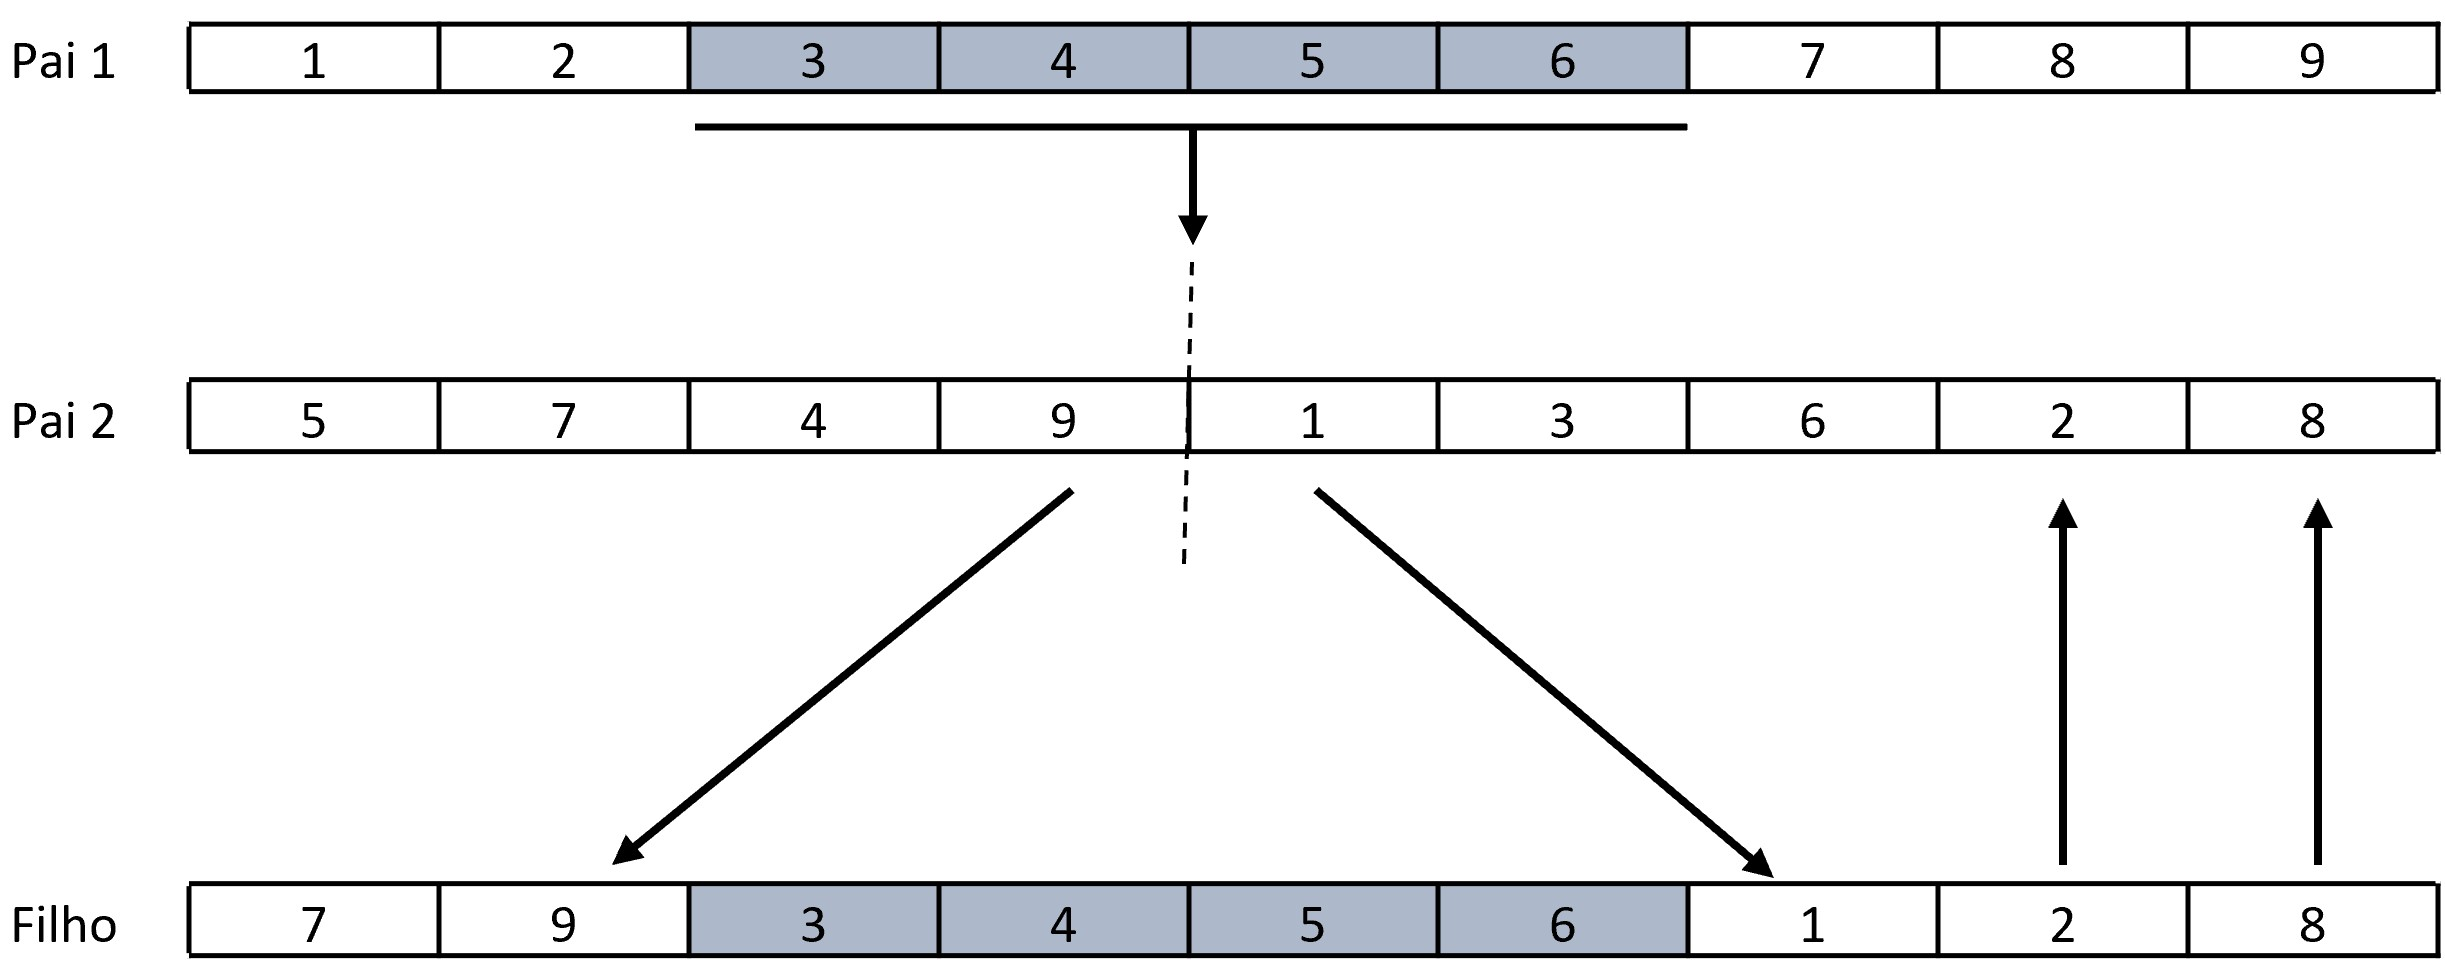
\includegraphics[width=.8\textwidth]{order_crossover.jpg}
    \caption{O funcionamento do Order Crossover (adaptado de \cite{misc:geneticOperations})}
    \label{fig:orderCrossover}
\end{figure}

Dependendo da estrutura de dados e o algoritmo utilizado, uma rota\c{c}\~{a}o pode levar \`{a}
copia de todos os elementos de um \textit{container} para outro, tendo em vista que, por exemplo,
um vetor somente permite a inser\c{c}\~{a}o de elementos em somente uma extremidade. Este
comportamento pode tornar esta simples tarefa uma, rotina de complexidade $\mathcal{O}(n)$.

Entretanto esta complexidade pode ser reduzida simplesmente utilizando uma estrutura do tipo
\textit{Deque} (\textit{Double-Ended Queue}). Esta estrutura de dados permite que sejam inseridos
elementos por ambos os lados, permitindo a rota\c{c}\~{a}o dos elementos com complexidade
$\mathcal{O}(1)$ com f\'{a}cil implementa\c{c}\~{a}o.

Vale ressaltar que a estrutura de \textit{hash} n\~{a}o suporta ordena\c{c}\~{a}o, ent\~{a}o
ainda \'{E} necess\'{a}rio utilizar um vetor para guardar os valores gerados. Esta decis\~{a}o
aumenta o consumo de mem\~{a}ria RAM mas pode diminuir consideravelmente o tempo de processamento.

\subsection{Gera\c{c}\~{a}o aleat\'{o}ria de elementos n\~{a}o repetitivos}\label{sec:nonRepeating}

Ao inicializar uma popula\c{c}\~{a}o de indiv\'{i}duos aleatoriamente, em muitos casos existe
a necessidade de um indiv\'{i}duo n\~{a}o possuir genes com valores repetidos. Ou seja, a cada novo
elemento inserido com um valor aleat\'{o}rio, deve-se certificar se o mesmo j\'{a} foi inserido
anteriormente. Caso positivo, devem ser gerados valores aleat\'{o}rios at\'{e} que esta
condic\c{c}\~{a}o se torne falsa, e ent\~{a}o o elemento \'{e} inserido no cromossomo do indiv\'{i}duo.

Como pode-se perceber, podem ser necess\'{a}rias muitas buscas sucessivas no vetor de genes para verificar
a exist\^{e}ncia de um elemento. A complexidade desta opera\c{c}\~{a}o geralmente \'{e} $\mathcal{O}(n)$,
por\'{e}m nesta situa\c{c}\~{a}o, o valor de n \'{e} incrementado por um a cada elemento que \'{e} inserido
neste vetor. O n\'{u}mero de buscas realizadas nesta situa\c{c}\~{a}o \'{e} dado pela
Equa\c{c}\~{a}o~\ref{eq:numNatural}, onde n \'{e} o n\'{u}mero m\'{a}ximo de genes do indiv\'{i}duo. A partir
deste fato, conclui-se que a complexidade algor\'{i}mica da gera\c{c}\~{a}o de todos os genes \'{e} de
$\mathcal{O}(n^2)$.

\begin{equation}
    \frac{n(n+1)}{2}
    \label{eq:numNatural}
\end{equation}

\'{E} muito importante otimizar esta etapa do processo, porque ela \'{e} executada inicialmente m vezes, sendo
m o tamanho da popula\c{c}\~{a}o. Realizar uma implementa\c{c}\~{a}o ineficiente ocasionar\'{a} um aumento de
tempo para computar os resultados, independentemente do qu\~{a}o eficiente seja a heur\'{i}stica durante a etapa
de evolu\c{a}\`{a}o.

Uma das op\c{c}\~{o}es para solucionar este problema \'{e} adotar uma estrutura de \textit{hash} para armazenar os
elementos j\'{a} inseridos. Para este tipo de estrutura, \'{e} adotada uma fun\c{c}\~{a}o que recebe uma entrada e,
numa situa\c{c}\~{a}o ideal, produz uma sa\'{i}da exclusiva para esta determinada entrada. Desta maneira, \'{e}
poss\'{i}vel verificar a exist\^{e}ncia de um elemento no \textit{container} sem a necessidade de verificar todas
as entradas anteriores. Desta forma, a complexidade algor\'{i}tmica \'{e} reduzida para $\mathcal{O}(1)$.

\subsection{Gera\c{c}\~{a}o alet\'{o}ria de subvetores}

Em alguns casos de uso, os genes do ind\'{i}viduo podem ser agrupados, a fim de atender a um sentido logico do problema
o qual esta sendo modelado. Por exemplo, quando se modela o ind\'{i}viduo para resolver o Problema de Roteamento de
Ve\'{i}culos (PRV), \'{e} comum inserir genes adicionais que dizem respeito as posi\c{c}\~{o}es do vetor que contem a primeira
localiza\c{c}\~{a}o da rota.

Na Figura~\ref{fig:vrpGenes}, o cromossomo indiv\'{i}duo pode ser divido em duas partes: a ordem das localiza\c{c}\~{o}es
a serem visitadas e os pontos de quebra do vetor para separa\c{c}\~{a}o das rotas. Note que a segunda parte cont\'{e}m os
indices do vetor onde \'{e} iniciada a representa\c{c}\~{a}o de uma nova rota.

\begin{figure}[ht]
    \centering
    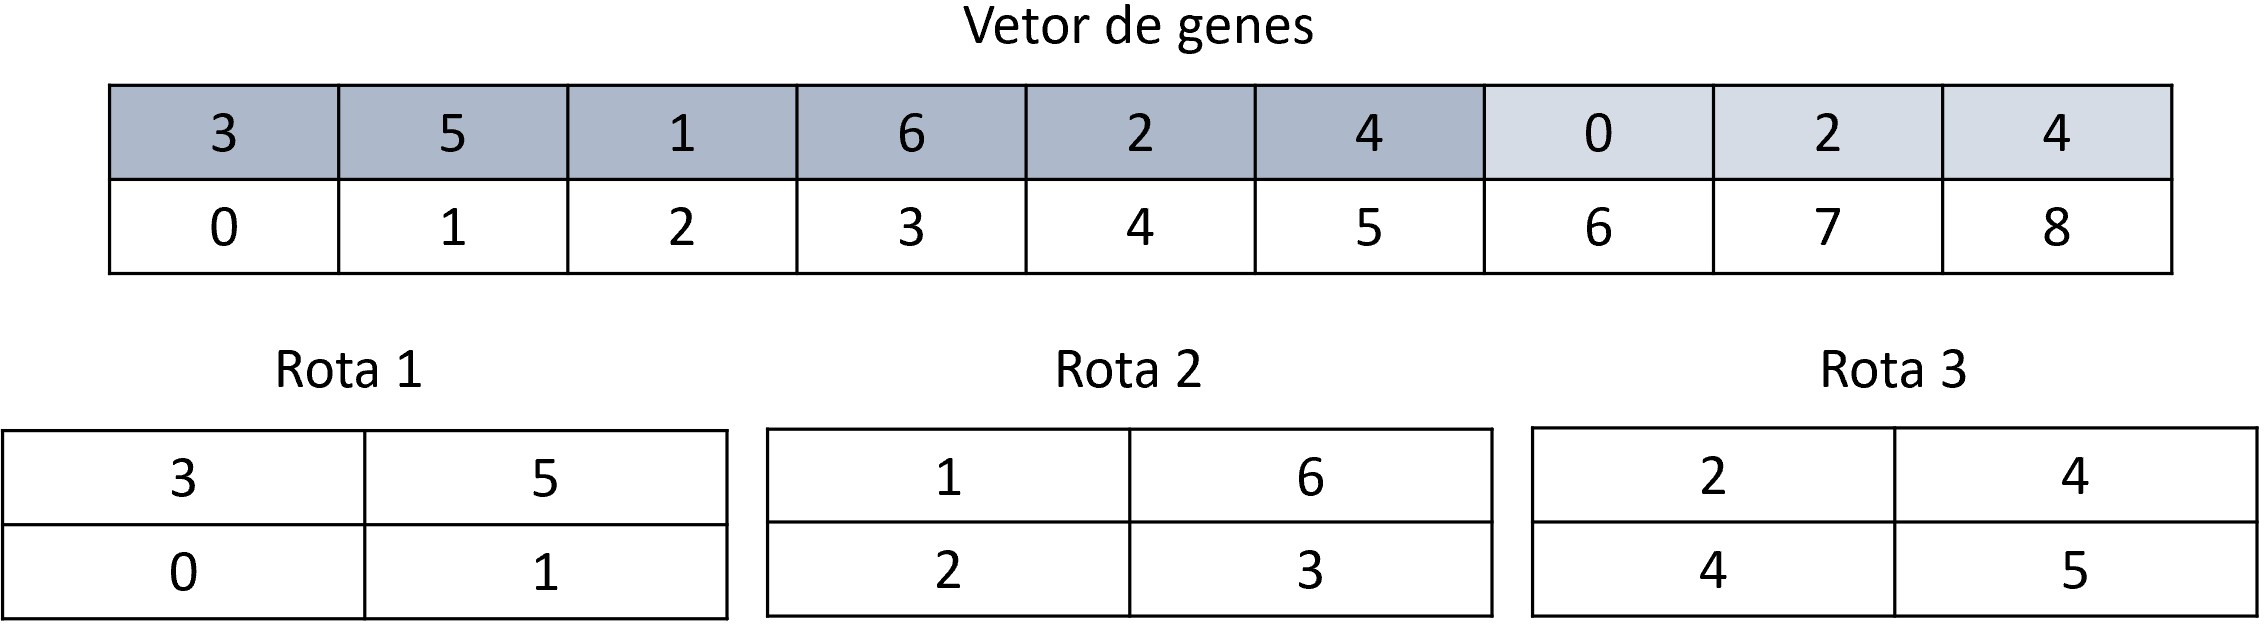
\includegraphics[width=.8\textwidth]{vrp_genes.jpg}
    \caption{Modelagem de um indiv\'{i}duo para o PRV}
    \label{fig:vrpGenes}
\end{figure}

Como visto na se\c{c}\~{a}o~\ref{sec:nonRepeating} \'{e} poss\'{i}vel utilizar uma estrutura de \textit{hash} para
acelerar o processo de busca de um elemento, mas ainda \'{e} necess\'{a}rio utilizar um vetor, porque o
\textit{hash} n\~{a}o \'{e} uma estrutura ordenada. Por\'{e}m para gerar a segunda parte deste vetor, \'{e} necess\'{a}rio que
os elementos gerados estejam em ordem crescente. Deste modo, ainda seria preciso executar um
algoritmo de ordena\c{c}\~{a}o ap\'{o}s a gera\c{c}\~{a}o dos elementos.

Para evitar esta etapa, uma solu\c{c}\~{a}o seria substituir o vetor por uma estrutura de \'{a}rvore ordenada. Existem
alguns tipos de \'{a}rvores ordenadas, e uma das mais utilizadas \'{e} a \'{a}rvore Rubro-Negra, devido \`{a} sua
capacidade de auto-balanceamento e garantia de busca de um elemento com complexidade $\mathcal{O}(\log_2n)$.
Assim \'{e} poss\'{i}vel armazenar os valores gerados em ordem enquanto s\~{a}o gerados.

Dependendo da quantidade m\'{a}xima de elementos deste vetor aleat\'{o}rio, utilizar somente uma \'{a}rvore pode
ser o suficiente para adquirir um desempenho aceit\'{a}vel. Mas ainda \'{e} poss\'{a}vel utilizar um \textit{hash}
auxiliar para acelerar verifica\c{c}\~{a}o de exist\^{e}ncia de um elemento. Assim a complexidade desta etapa seria
reduzida de $\mathcal{O}(\log_2n)$ para $\mathcal{O}(1)$.

\section{Implementa\c{c}\~{a}o}

Como existe uma grande quantidade de estruturas de dados existentes e cada uma possui pontos fortes e fracos,
\'{e} comum que se utilize em um projeto de software uma grande variedade delas, a fim de extrair a melhor utilidade
de cada uma. Entretanto, se fosse necess\'{a}rio implement\'{a}-las manualmente, o projeto se tornaria muito mais
demorado e talvez at\'{e} invi\'{a}vel. Al\'{e}m disso, muitas destas estruturas possuem implementa\c{c}\~{o}es
complexas e muitas vezes n\~{a}o se consegue alcan\c{c}ar o desempenho esperado com uma implementa\c{c}\~{a}o manual
porque \'{e} preciso muito tempo para refatorar o c\'{o}digo at\'{e} que ele alcance tal n\'{i}vel de efici\^{e}ncia.

Por estes motivos, \'{e} importante utilizar as estruturas de dados dispon\'{i}veis na biblioteca padr\~{a}o da linguagem
utilizada. O projeto da biblioteca padr\~{a}o \'{e} mais maduro e j\'{a} foi testado muitas vezes para garantir sua
efici\^{e}ncia, al\'{e}m de ser praticamente livre de \textit{bugs}. Todas as estruturas de dados citadas neste artigo
est\~{a}o dispon\'{i}veis na linguagem C++. Muitas delas tamb\'{e}m est\~{a}o dispon\'{i}veis em outras linguagens de
programa\c{c}\~{a}o, como Python e Java.

Mesmo que esta estrutura n\~{a}o esteja dispon\'{i}vel na linguagem de programa\c{c}\~{a}o desejada e n\~{a}o exista
uma solu\c{c}\~{a}o similar, pode-se optar por bibliotecas de terceiros que realizem esta implementa\c{c}\~{a}o. Apesar deste
m\'{e}todo n\~{a}o garantir um projeto eficiente e livre de \textit{bugs}, ainda \'{e} uma op\c{c}\~{a}o mais segura
do que realizar a implementa\c{c}\~{a}o manual.

Caso a pessoa esteja disposta a colaborar com o desenvolvimento de uma biblioteca de estrutura de dados, existem
diversos resposit\'{a}rios de c\'{o}digo aberto dispon\'{i}veis na internet. Assim, a pessoa tem a chance de
colaborar com uma equipe em um projeto que tem um potencial de ajudar muitos desenvolvedores.

\section{Conclus\~{a}o e trabalhos futuros}

Atrav\'{e}s deste texto foi poss\'{i}vel compreender o conceito de algumas estruturas de dados utilizadas
atualmente, al\'{e}m de conhecer algumas aplica\c{c}\~{o}es para elas. \'{E} de suma import\^{a}ncia escolher a estrutura
de dados mais adequada para resolver o problema e em quest\~{a}o, para garantir melhor efici\^{e}ncia e talvez at\'{e}
permita que o c\'{o}digo seja mais limpo e com menos rotinas.

Quando se trata de intelig\^{e}ncia computacional, \'{e} importante que o c\'{o}digo seja eficiente, porque muitas
vezes se lida com um grande volume de dados. Seguindo algumas t\'{e}cnicas mostradas neste artigo, foi poss\'{i}vel
reduzir a complexidade de tarefas de linear e quadr\'{a}tica para constante, podendo reduzir consideravelmente o tempo de
execu\c{c}\~{a}o do algoritmo.

Apesar de este artigo ter sido escrito sob a implement\c{c}\~{a}o de um algoritmo gen\'{e}tico, nele n\~{a}o est\~{a}o
presentes os testes de desempenho para verificar se houve um ganho real ao optar por estas estruturas de dados.\'{E} esperado
que haja uma melhora devido ao fato de algumas opera\c{c}\'{o}es serem otimizadas. Futuramente pode ser feito um novo
trabalho sobre este tema abordando os ganhos em tempo de execu\c{c}\'{a}o ao utilizar estas estruturas.

\bibliographystyle{sbc}
\bibliography{sbc-template}

\end{document}
